\documentclass[14pt]{extarticle}
\usepackage{graphicx}
\usepackage{hyperref}
\usepackage[english]{babel}
\usepackage[final]{pdfpages}

\usepackage[utf8x]{inputenc}
\usepackage{listings}
\usepackage{xcolor}
\usepackage{color}




\definecolor{javared}{rgb}{0.6,0,0} % for strings
\definecolor{javagreen}{rgb}{0.25,0.5,0.35} % comments
\definecolor{javapurple}{rgb}{0.5,0,0.35} % keywords
\definecolor{javadocblue}{rgb}{0.25,0.35,0.75} % javadoc
 
\lstset{language=Python,
    keywordstyle=\color{javapurple},
    basicstyle=\small,
    commentstyle=\color{javagreen},
    stringstyle=\color{javadocblue},
    showstringspaces=false,
    breaklines=true,
    frameround=ffff,
    frame=single,
    rulecolor=\color{black}
} 


\begin{document}
\title{
\includegraphics{download.jpeg} \vspace{2cm} \textbf{\\Parameter Learning in una rete bayesiana}}

\author{\texttt{Pietro Bernabei} - \texttt{matricola:6291312}\\ \texttt{Anno Accademico 2019/20}}
\date{}
\maketitle

\newpage
\section{Introduzione}
	Il progetto è stato sviluppato su Python 3.8, ed è composto da due componenti, la cartella\textbf{Data}, il file python \textbf{progetto.py}.
	La cartella \textbf{Data}, contiene modelli di rete bayesiane, definite all'interno del progetto di \textbf{ncullen93}, 	\textbf{pyBN}. Qui sono state copiate per permettere un più facile accesso.
	Il programma è impostato per essere eseguito sulla rete bayesiana \textbf{asia.bif} generando un dataset di 2000 elementi, di cui con quantità crescente viene fatta apprendere alla rete\\\\
	\section{Installazione}	
Mentre per l'installazione del progetto LearningParameter:
\begin{lstlisting}
git clone https://github.com/BernabeiPietro/LearningParameter.git
cd LearningParameter
conda env create -f environment.yml
\end{lstlisting}

	\section{Esecuzione}
		Entrare nella cartella principale e eseguire il file main.py con il comando:
		\begin{lstlisting}
		python3 main.py
		\end{lstlisting}
		
	\section{Risultati}
	Di seguito si porta le curva di apprendimento ottenute da 2 diverse esecuzione, le quali sono simili, tranne per qualche leggera differenza, siccome il training set viene ogni volta ricalcolato.\\
	Nel caso si volesse visionare  i valori della rete durante l'esecuzione del programma è necessario modificare la variabile printBN del file progetto.py in True\
	\begin{figure}[t]
	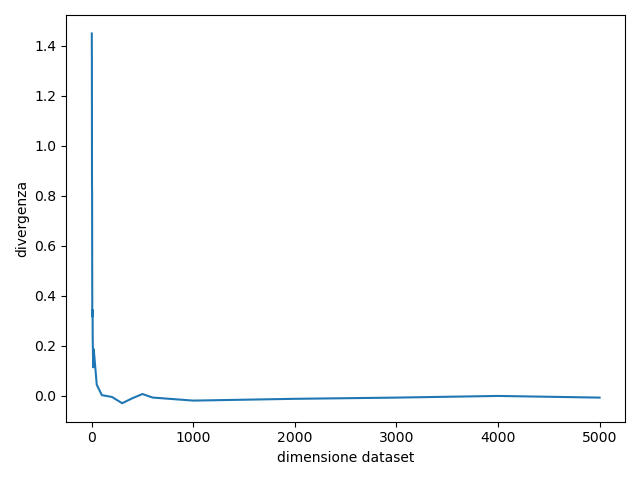
\includegraphics[scale=0.8]{Figure_1.png}\\
	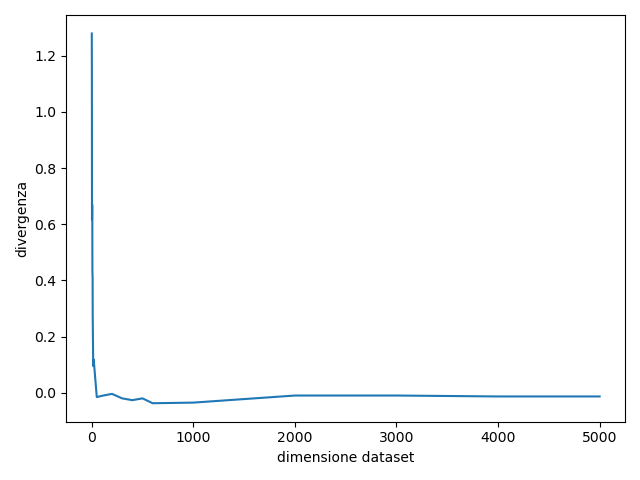
\includegraphics[scale=0.8]{Figure_2.png}\\
	\centering
	\end{figure}
	
\end{document}

